\chapter{Problem formulation}

%IDEAL
This thesis considers the problem of autonomous USV maneuvering for complete bathymetric coverage of the seabed. The USV workspace is assumed to be a bounded rectangular 2D region, with possibly the presence of obstacles. The maneuvering system generates continuous steering control that allows the USV to \emph{efficiently} cover the seabed with its observation sensor, i.e. reducing undesired overlapping sensor coverage. Obstacles within the target region are avoided. The system operates with no prior knowledge of the target region.

%REALITY
Most existing complete coverage algorithms are offline and covers the target region using boustrophedon motions, and the spacing between the back-and-forth laps is determined by the coverage range of the robot's sensor or end-effector. However, when covering the seabed while navigating on the surface, the observation sensor's coverage range varies depending on the water depth. Consequently, existing complete coverage methods that are aimed towards land-based robots such as vacuum cleaners or lawnmowers with a constant coverage range, cannot directly be applied to USVs. There are works in the literature that consider varying coverage range due to water depth, for both ASVs and AUVs operating at constant depth. However, online approaches that also consider obstacles in the target region are still left largely unexplored.

%SOLUTION
The USV is assumed to be a Dubins vehicle, i.e. a non-holonomic vehicle that is constrained to move along planar paths of bounded curvature, and can only travel forward along the path. The observation sensor is a multibeam echosounder that covers the seabed in a swath directly beneath the USV and perpendicular to the moving direction. The swath extends a distance $c_p$ and $c_s$ in the port and starboard directions, respectively. A low-cost 2D lidar is mounted on top of the USV and used to detect and avoid obstacles on the surface. Moving obstacles can be considered as long as they move slowly compared to the USV. The system fuses information from lidar, IMU, and GNSS in order to maintain an always up-to-date map of obstacles in the surrounding environment. The map is partitioned into a grid, which is used by a path planning method to plan collision-free paths that ensure complete coverage of the seabed. These generated paths consist of a series of waypoints, and are further processed in order to generate feasible trajectories using simple Dubins paths. These trajectories take into account the turning radius, speed, and maximum stopping distance of the USV. Lastly, these trajectories are fed into a path following controller that generates continuous course and speed control that are passed to the Otter USV's onboard systems. A topology drawing of the control system and its information flow is shown in \figref{fig:topology}. Maritime Robotics' already existing systems, which need to be interfaced with, are marked in the figure.

\begin{figure}[h!]
	\centering
	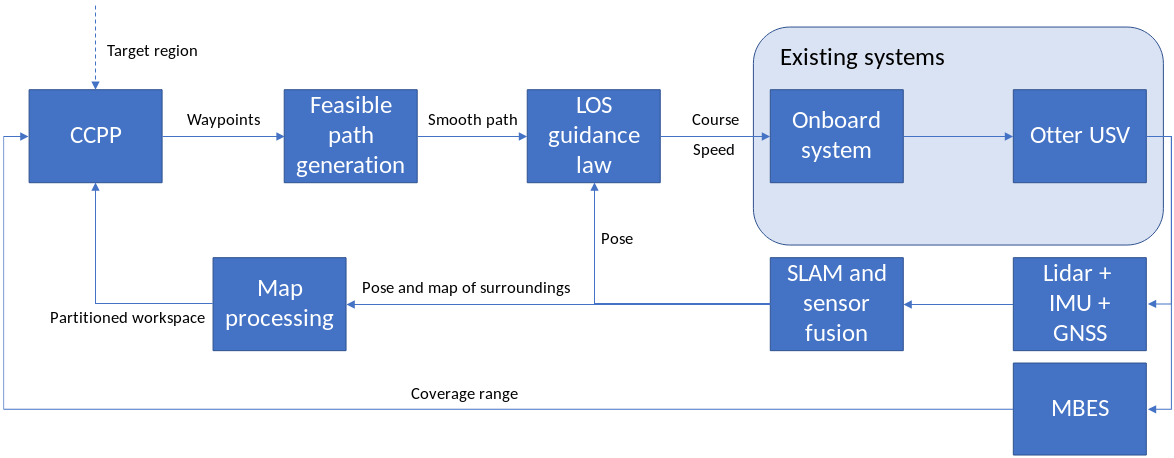
\includegraphics[width=1.0\linewidth]{fig/topology}
	\caption{The control system and its information flow.}
	\label{fig:topology}
\end{figure}
